
\chapter{Использование программы}
Главное окно программы состоит из двух вкладок: “Условия” и “Решение”.
В первой вкладке осуществляется ввод условий задачи. Во второй вкладке отображается ход решение и результат.
Внешний вид и оформление программы могут отличаться в зависимости от платформы, на которой будет запущена программа.

\begin{figure}[ht]
\centering
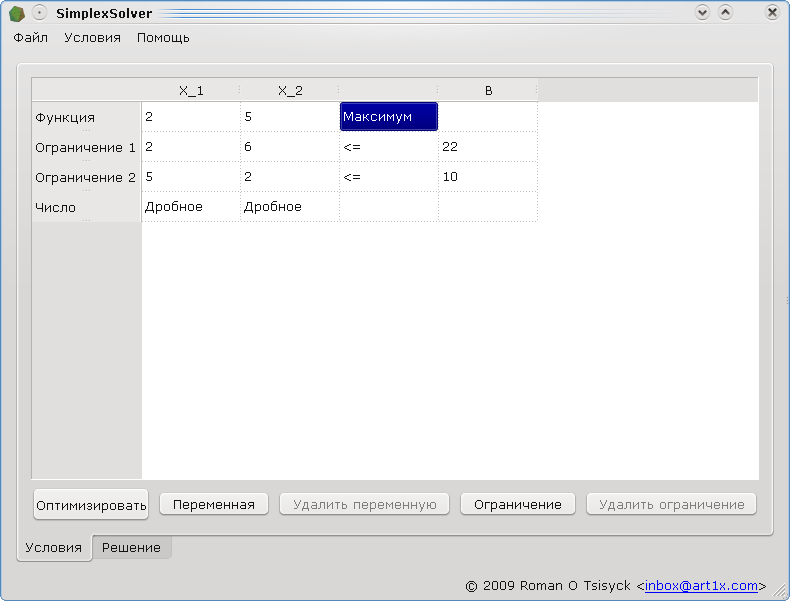
\includegraphics[width=\textwidth]{img/mainwindow.png}
\caption{Главное окно программы}
\end{figure}
\clearpage

\section{Ввод задачи}
Во вкладке “Условия” в первой строке необходимо задать целевую функцию (вектор-строка $\vec{C}$ и тип оптимизации.
Во всех остальных строках, кроме последней, наобходимо задать коэффициенты матрицы, знаки неравенств и значение свободных членов системы ограничений. В последней строке задаются ограничения целочисленности каждой из переменных.

Для добавления переменных и ограничений можно воспользоваться кнопками cнизу таблицы или контекстным меню (на правую клавишу мыши).
\begin{figure}[ht]
\centering

\includegraphics[scale=1.0]{img/contextmenu.png}
\caption{Контекстное меню таблицы}
\end{figure}

Пример. Задача задана в следующем виде:
\begin{equation}
 	F(\vec{X}) = x_1+x_2 \to max,
\end{equation}
\begin{equation}
\begin{cases}
x_1 + 5x_2 \le 10\\
7x_1 + 8x_2 \le 4\\
x_i \ge 0.
\end{cases}
\end{equation}
\clearpage
В окне программы это будет выглядеть следующим образом:
\begin{figure}[ht]
\centering
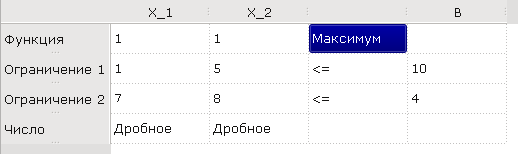
\includegraphics[scale=1.0]{img/problem1.png}
\caption{Задание условий задачи в программе}
\end{figure}

\section{Получение решения}
Во вкладке “Решение” отображается ход решения. В начале документа показана задача, приведенная к каноническому виду.

\begin{figure}[ht]
\centering
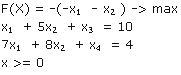
\includegraphics[scale=1.0]{img/canonical.png}
\caption{Задача в каноническом виде}
\end{figure}

Далее идут промежуточные симплекс-таблицы, которые могут быть полезны для понимания механизма работы алгоритма или более детального исследования задачи. Следует учитывать, что при нахождении максимума, оценки в $m+1$ и $m+2$ строках таблицы записаны с противоположными знаками. При отсутствии искусcтвенных переменных, $m+2$ строка не отображается.

\begin{figure}[hb]
\centering
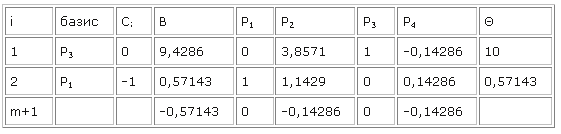
\includegraphics[scale=1.0]{img/simplextable.png}
\caption{Симплекс-таблица}
\end{figure}
После таблиц отображается оптимальное значение функции $F(\vec{X})$ и значения соотвествующих переменных $x_{i}$ ввиде компонентов вектора $\vec{X}$.

\newpage
\clearpage

\begin{figure}[ht]
\centering
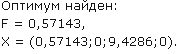
\includegraphics[scale=1.0]{img/result.png}
\caption{Результат}
\end{figure}

В самом конце указаны интервалы устойчивости $\vec{С}$ и $\vec{B}$, при которых двойственные оценки сохраняют свое значение.
\begin{figure}[hb]
\centering
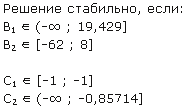
\includegraphics[scale=1.0]{img/stability.png}
\caption{Интервалы устойчивости}
\end{figure}

\section{Сохранение результата}
Вывод программы можно сохранить в файл. В данной версии поддерживается формат OpenDocument Text (.odt), который в свою очередь может быть открыт популярным офисным пакетом OpenOffice.org, и формат HTML 4 (.html), который может быть просмотрен любым совместимым веб-браузером. Предусмотрена возможность отправки вывода программы на печать.
